\clearpage
\section{Sample selection}
\label{sec:Sample_selection}

\subsection{COSMOS field}

\begin{table}[htbp]

	\hspace{50pt}

	\begin{tabular}{ccccccc}
	\hline
	Group & Ra\textsuperscript{2} & Dec\textsuperscript{3} & Exposure\textsuperscript{4}  & Average & Total nb. & Nb. field \\
	
	ID\textsuperscript{1} & J2000 (\degree) & J2000 (\degree) & (hr) & seeing\textsuperscript{5} (") & galaxies\textsuperscript{6} & galaxies\textsuperscript{7} \\	
	
	\hline
	\hline
	CGr32 & NaN & NaN & $3 \times 4.35$ & $0.51$ - $0.58$ & NaN & NaN \\
	\hline
	CGr34\_d & $149.87766$ & $2.502331$ & $5.25$ & $0.63$ & NaN & NaN \\
	\hline
	CGr34\_bs & $149.87766$ & $2.502331$ & $4.75$ & NaN & NaN & NaN \\
	\hline
	CGr30\_d & $150.144225$ & $2.065971$ & $9.75$ & $0.67$ & NaN & NaN \\
	\hline
	CGr30\_bs & $150.144225$ & $2.065971$ & $6.25$ & NaN & NaN & NaN \\
	\hline
	CGr84 & $150.057219$ & $2.599744$ & $5.25$ & $0.59$ & NaN & NaN \\
	\hline
	CGr84-N & NaN & NaN & $1$ & $0.51$ & NaN & NaN \\
	\hline
	CGr114 & $149.994285$ & $2.258044$ & $2.2$ & $0.68$ & NaN & NaN \\
	\hline
	CGr79 & $149.820686$ & $1.821825$ & $4.35$ & $0.60$ & NaN & NaN \\
	\hline
	CGr28 & $150.218094$ & $1.812667$ & $1$ & $0.62$ & NaN & NaN \\
	\hline
	CGr26 & $150.492767$ & $2.069139$ & $1$ & $0.59$ & NaN & NaN \\
	\hline
	CGr61 & $149.728741$ & $1.915987$ & $1$ & $0.64$ & NaN & NaN \\
	\hline
	CGr51 & $149.982756$ & $1.801899$ & $1$ & $0.6-0.7$ & NaN & NaN \\
	\hline
	CGr23 & $149.790782$ & $2.162648$ & $1$ & $0.68$ & NaN & NaN \\
	\hline
	
	\end{tabular}
	
	\caption[Main characteristics of the observed MUSE fields]{\label{table:MUSEfieldsProp}Main characteristics of the observed MUSE fields. Groups ending with \_d correspond to deep observations (full stacked OBs) and with \_bs correspond to best-seeing observations (only OBs with a seeing below $\SI{0.7}{"}$). The seeing is given for the OII wavelength at the group's redshift. 1. MUSE group number, 2. Group centre's right ascension, 3. Group centre's declination, 4. Duration of observations, 5. Average seeing during observation, 6. Total number of detected galaxies within MUSE FoV, 7. Number of field galaxies found by the FoF algorithm.}
\end{table}

The point of the analysis is to perform a joint study of the morphology and the kinematics of field galaxies in the COSMOS field using respectively HST ACS images and MUSE data. To this end, a set of 9 galaxy groups in the COSMOS field was selected. The choice of the COSMOS field for this analysis was made because of the large number of multi-band photometric data available for the galaxies in this field and the presence of rich (large number of member galaxies) galaxy groups.\\

Guaranteed Time Observation (GTO) runs centred on those groups were performed from which 13 different MUSE Fields of View (FoV) of $1 \times \SI{1}{arcsec^2} $ were obtained. Each group corresponds to one FoV, except for the group number 32. Since it is larger than the others, three different observations were carried out around it with a slight overlapping (mosaic view) between them. The main characteristics of the observed FoVs, including the position of their centre, the number of observing time hours, the average seeing during the observation, the total number of galaxies and the number of field galaxies detected by the FoF algorithm are listed in Table\,\ref{table:MUSEfieldsProp}.

These groups were primarily chosen for their position within the COSMOS field. This ensured them to have a large set of corresponding photometric data available from \shortciteA{laigle_cosmos2015_2016} catalogue for most of the galaxies. Nevertheless, since blind source detections within the data cubes were performed on these FoVs, we should expect a small fraction of galaxies to be detected in MUSE cubes but not in the HST images.\\

Generally speaking, galaxies detected by MUSE are also detected in HST images because of the Hubble Space Telescope's (HST) much better resolution (\SI{0.03}{arcsec/px} for HST and $\sim \SI{0.2}{arcsec/px}$ for MUSE). Nevertheless, the MUSE pipeline allows in some cases the detection of sources in regions where there is no HST counterpart. Two sources can even be separated in areas smaller than the PSF based on their different spectral features, though this happens not often \shortcite{sourceDetectionMUSE}.

\subsection{Prior information on the galaxies}

\subsubsection{Cluster galaxies}

This internship was planned to be similar in many aspects to what has been doing Epinat B. PhD student Valentina Abridg in LAM, Marseille for her PhD. Her work consisted in studying the morphology and the kinematics of the galaxies within the structures observed by MUSE. The galaxies she was working on were therefore found in the same FoVs but belonged to groups and clusters when those I used were labelled as field galaxies around these structures. 

To differentiate between group and field galaxies, prior to my arrival, a Friend of Friends algorithm (FoF) was run on the galaxies in each FoV in order to separate them into two categories: group and field galaxies.

Additionnaly, GalFit had been run on the cluster galaxies by Valentina and we therefore already had morphological information for them.
Unlike other software such as SExtractor or GIM2D which fit a one-component model (Sérsic index as a free parameter) onto the images, the morphological model which was used in this case used a combination of a disk component (Sérsic index $n=1$) and a spherically symmetric bulge component ($n=4$). 

Hence, we already had the following morphological parameters for the cluster galaxies only: ellipticity and PA (from the disk component), bulge and disk total magnitudes and the half-light radii for both components\footnote{Note this means the value of GalFit half-light radii can be quite different from that given by SExtractor or GIMD2D as shall be discussed in later sections. }

\subsubsection{Morphological information from COSMOS catalogues}

The total number of galaxies detected by MUSE in the COSMOS field is around $1000$. Roughly half of them belong to clusters and the other half are labelled as field galaxies. Among these galaxies, not all of them are useful to our study. Some may be too close to the edge of detection, others be too noisy with a low Signal to Noise Ratio (SNR), or too small to perform any relevant kinematical modelling. It is thus mandatory to apply a selection on our data set of field galaxies, first to save time for the analysis, but also to reduce errors which might increase if we have too poorly resolved data.

The second point is that we would like to perform a joint study of the morphology and the kinematics of these galaxies. The tools and the models for the kinematical modelling were already developed and are the same as those used by Valentina in her work. On the other hand, fitting morphological models with software such as GalFit or SExtractor require additional time. Hopefully for us, morphological modelling was already performed on the galaxies in the COSMOS field, so we could focus on the kinematical part. \\

Morphological information for all galaxies in the COSMOS field can be found in various catalogues\footnote{\url{https://irsa.ipac.caltech.edu/data/COSMOS/tables/morphology/}}. To start with, we decided to use the two most complete catalogues we could find, that of Tasca (maybe citation) and Cassata (maybe citation as well). Both catalogues contain morphological information including the central position of the galaxy, its half-light radius, concentration and asymmetry parameters, ellipticity, PA, and many more for roughly $232 000$ galaxies. 

To associate the already present data from \shortciteA{laigle_cosmos2015_2016} within our catalogue with theirs, we cross-matched our data with each catalogue separately and then with both using the right ascension $\alpha$ and declination $\delta$ of the centre of the galaxies, allowing for a maximum separation between the MUSE source and the closest source within Cassata's and Tasca's catalogues of $\SI{1}{arcsec}$ maximum. However, we should note that the centre position of the MUSE galaxies correspond to that of the corresponding source in \shortciteA{laigle_cosmos2015_2016} and should therefore be quite close to the value of the cross-matched galaxy since their photometry modelling was performed on the same data. \\

We performed this cross-matching for both field and cluster galaxies. The reason for cross-matching cluster galaxies when we are only interested in those in the field will be discussed in the following section.

\subsection{Checking catalogues values consistency}
\subsubsection{Reasons for checking catalogues}

\begin{figure}[H]
	\centering
	\begin{minipage}[c]{0.49\linewidth}
		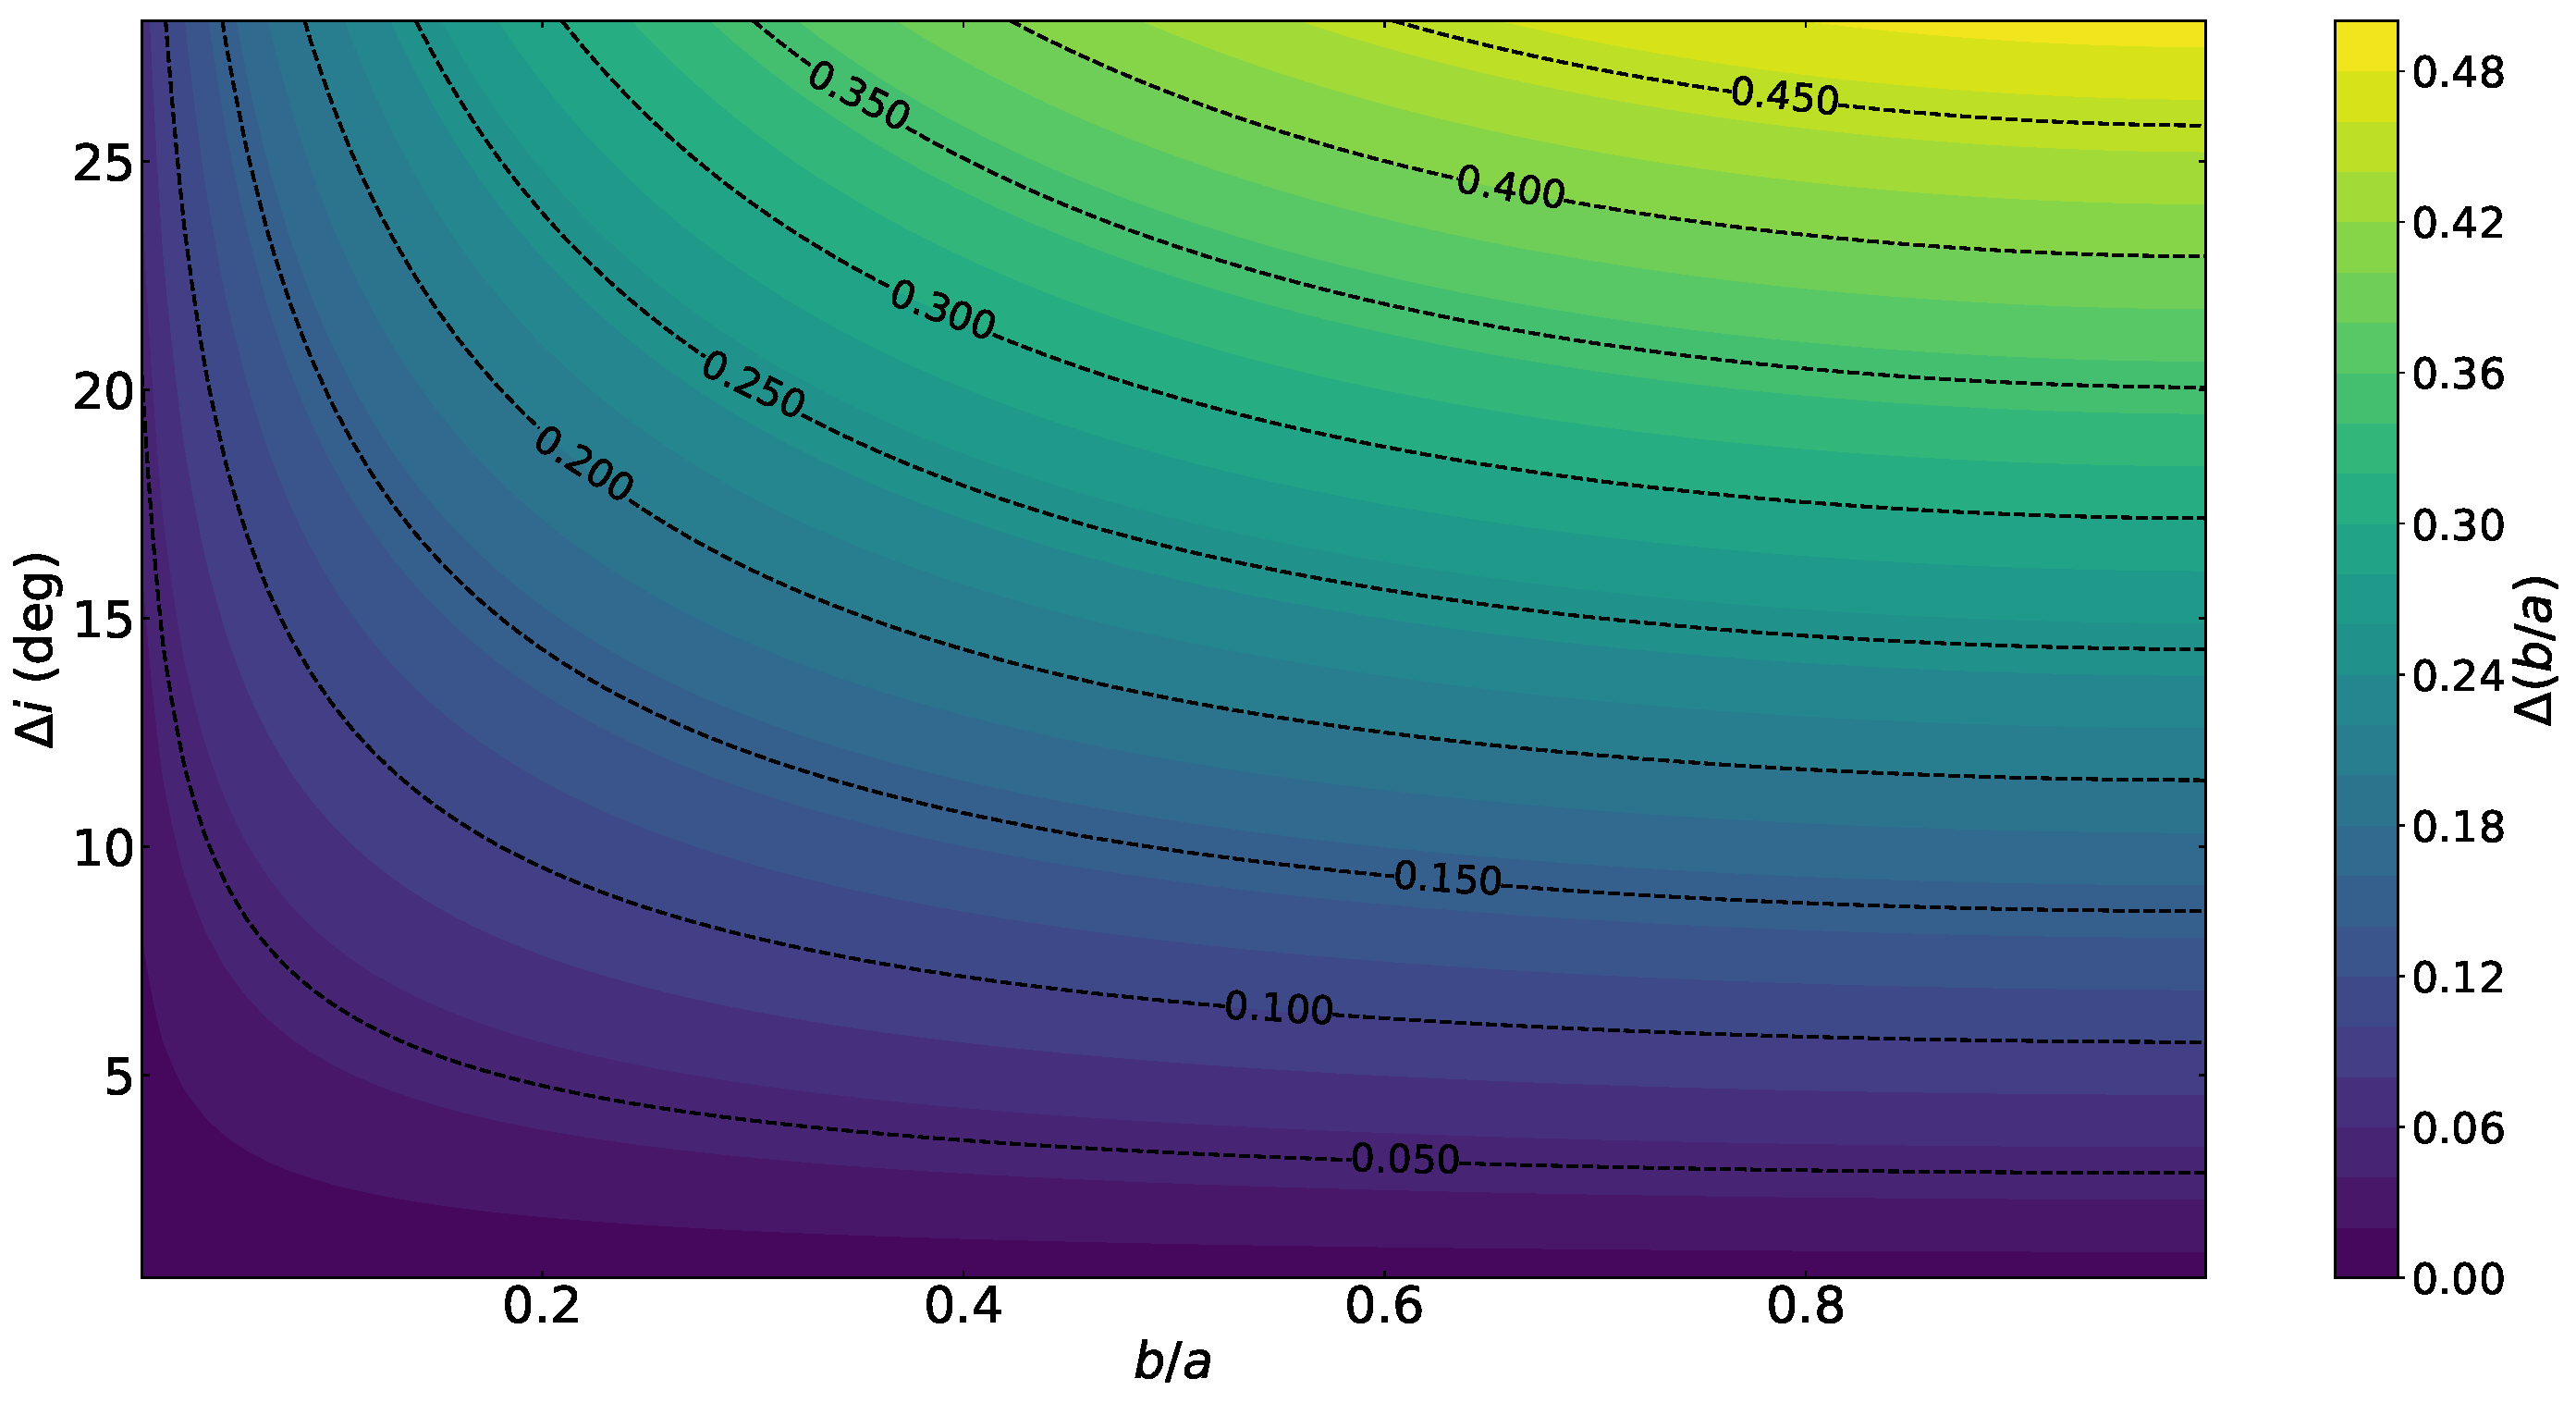
\includegraphics[width=\linewidth]{../Plots/Error_on_inc_versus_b_a.pdf}
		\subcaption{Error on inclination as a function of $b/a$ and its absolute error. Contours of $\Delta (b/a)$ are plotted in black dashed lines with their corresponding value.}
	\end{minipage}
	\hfill
	\begin{minipage}[c]{0.49\linewidth}
		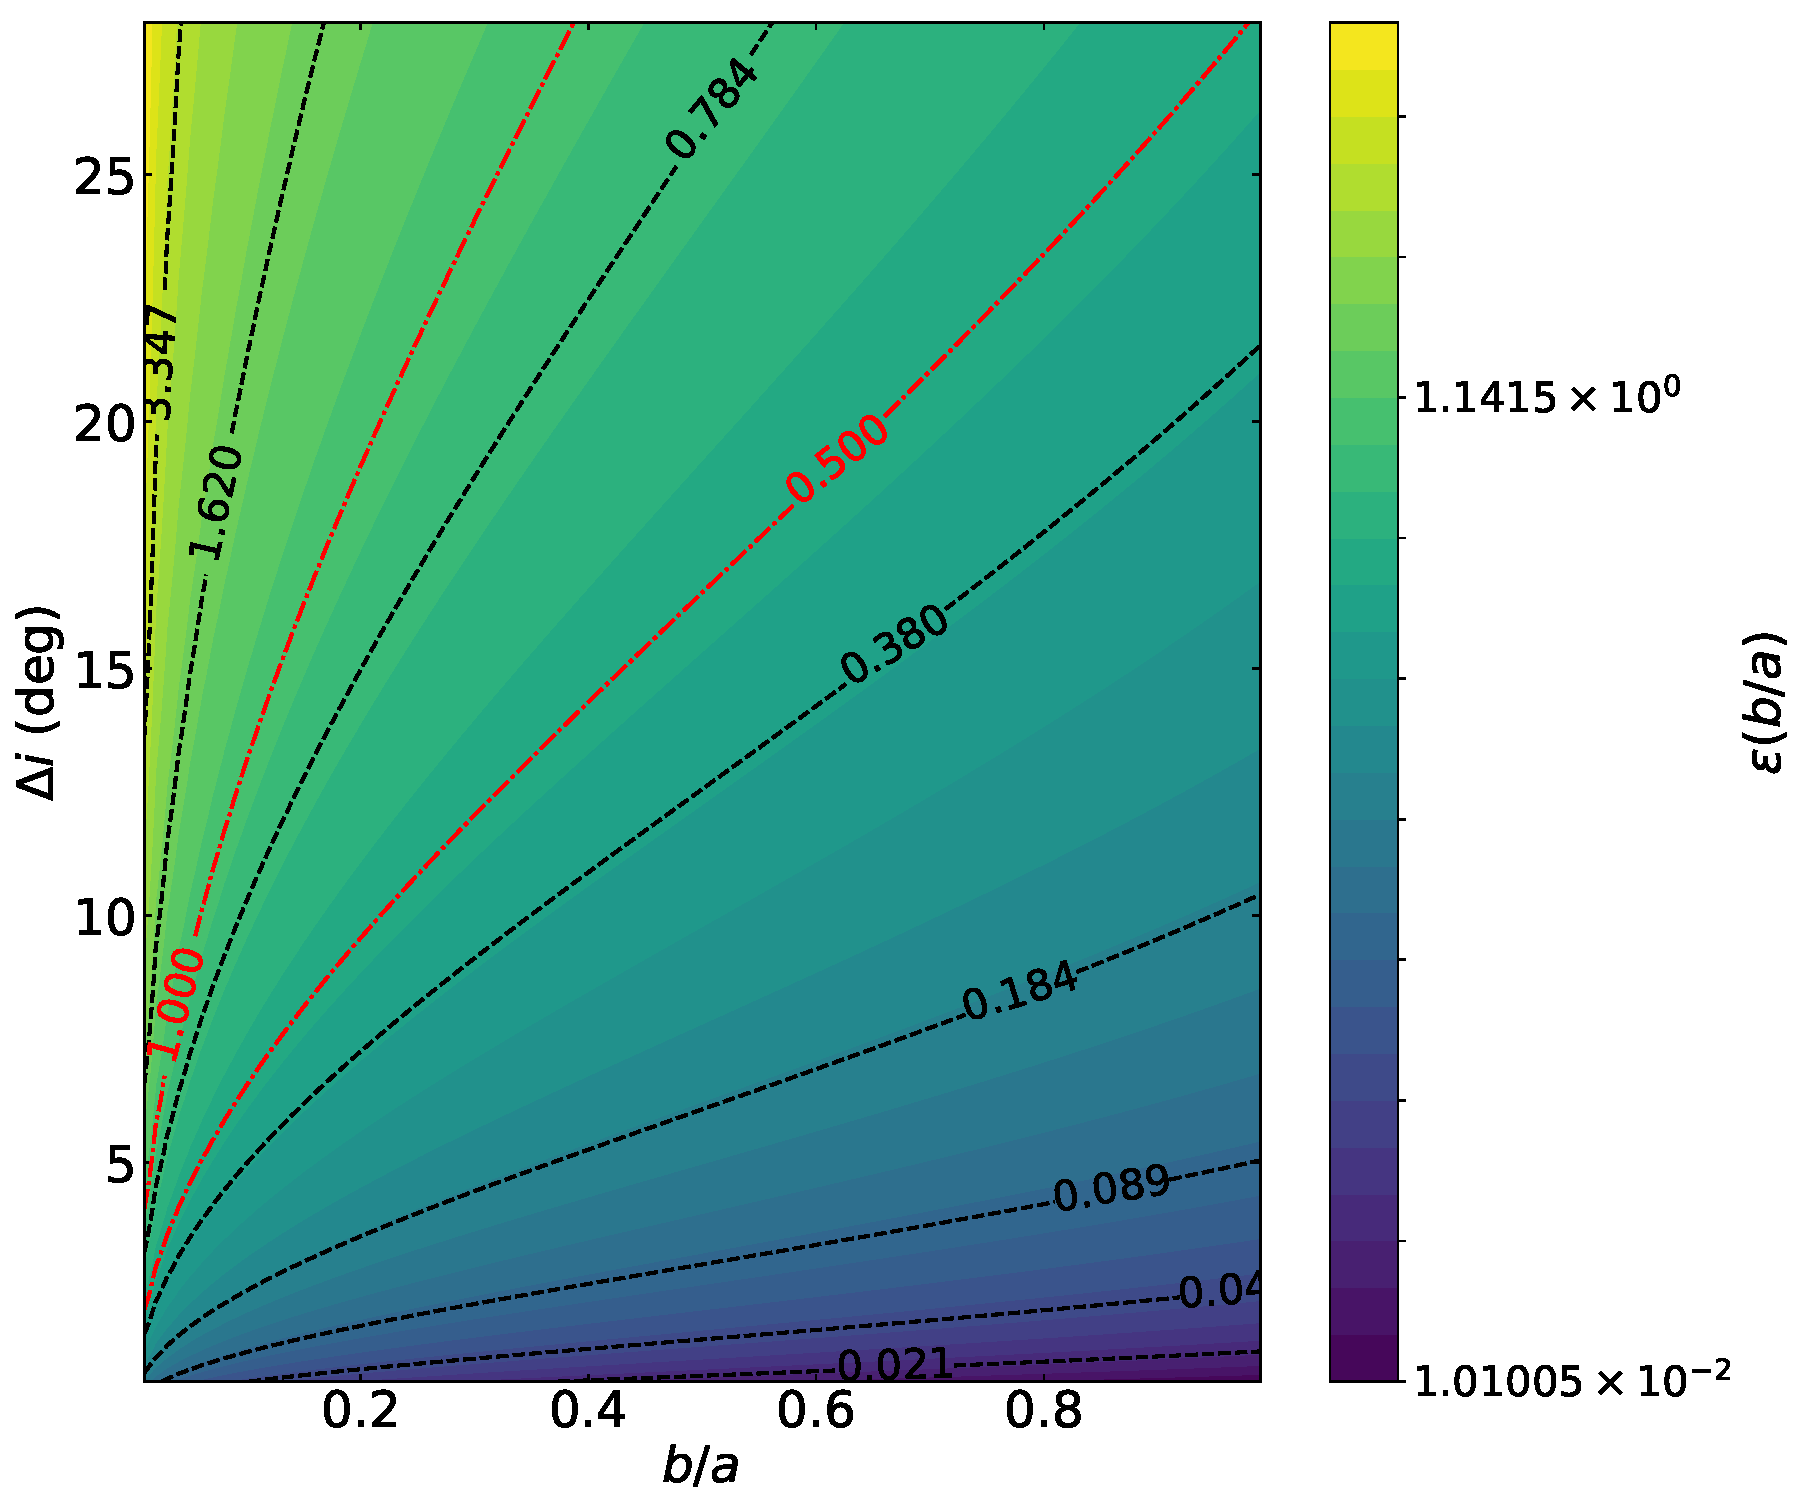
\includegraphics[width=\linewidth]{../Plots/RelError_on_inc_versus_b_a.pdf}
		\subcaption{Error on inclination as a function of $b/a$ and its relative error. Contours of $\epsilon (b/a)$ are plotted in black and red dashed lines with their corresponding value.}
	\end{minipage}
	\caption[Error on inclination as a function of $b/a$ and its error.]{Error on inclination as a function of $b/a$ and its error. Left: as a function of the absolute error on $b/a$ ($\Delta (b/a)$). Right: as a function of the relative error on $b/a$ ($\epsilon ( b/a)$). Red contours correspond to values for which there is a 50\% and 100\% error on $b/a$.}
	\label{fig:erreur_inclinaison}
\end{figure}

As in any analysis, we must select a sample based on relevant criteria to remove bad and/or uninteresting data for this work. This selection can only be done through morphological and overall spectral features since any kinematical modelling relies on prior morphological information. 

Before this internship, spectral fitting on the integrated spectra of the galaxies had already been done, and we knew we already had morphological information from COSMOS catalogues as discussed in the previous section. Potentially useful morphological information included the half-light radius, the magnitude, the ratio of minor to major axis ($b/a$) or equivalently a measure of the ellipticity of the galaxies. 

Nevertheless, using this data without checking first how well it compares to other values from other catalogues and/or measured via different softwares/methods could lead to high biases and uncontrolled errors. Thus, before discussing any selection criteria for our sample, we must first assess the reliability of the parameters we are going to use in later sections. \\

The three most important values for us are the half-light radius, as it will be used to select our sample, the total magnitude and the $b/a$ ratio. The last parameter has a crucial importance since it is directly related to the inclination of the galaxy on the sky through Eq.\,\ref{eq:inclinaison}. Given a certain error $\Delta (b/a)$ on the axes ratio, and using the usual formula for computing the error $\Delta f = | \partial_x f | \Delta x$ of a function $f(x)$, we find for the inclination

\begin{equation}
	\Delta i = \Delta (b/a) \left | \frac{b}{a} \left ( 2 - \frac{b}{a} \right ) \right | ^{-1/2}
\end{equation}

This is illustrated in Fig.\,\ref{fig:erreur_inclinaison} where $\Delta i$ has been plotted as a function of $b/a$ and its error (absolute on the left, relative on the right). Contours of the error on $b/a$ have been over-plotted to show how evolves $\Delta i$ given a fixed error on $b/a$. As expected, the higher the error on $b/a$ the higher the error on $i$. An error as high as 50\% could yield $\Delta i \approx \SI{27}{\degree}$, though this value is reached for $b/a \approx 1$ where it is the least constrained by the morphology. A more appropriate error on $b/a$ of 20\% gives a maximum $\Delta i$ slightly above $\SI{10}{\degree}$, which is correct. 

Since the inclination has an impact on the maximum rotational velocity, and so potentially on the classification of galaxies as rotationnaly supported or dispersion dominated (see Section insert ref here), this indicates us that for any proper kinematical modelling we must check carefully that the values of axes ratios are consistent between catalogues.

\subsubsection{Catalogues used for comparison}

As stated in previous sections, we cross-matched our catalogue of galaxies detected by MUSE in the COSMOS field with Cassata's and Tasca's, two tables with morphological information for the galaxies found in \shortciteA{laigle_cosmos2015_2016} catalogue. 

However, as this will be showed in the following paragraphs, it turned out that there were large discrepancies between the considered values. Thus, to better understand the origin of these discrepancies, we chose to cross-match a last time our catalogue with another one (also based on \shortciteA{laigle_cosmos2015_2016}) from Zurich. This table has fewer HST counterparts of MUSE galaxies than in the other two but it contains additional morphological information which we can use for the comparison. 

In addition to that, we already had morphological information from GALFIT fits on $\sim 500$ group galaxies, and we had strong confidence in the returned morphological values. Therefore, we chose to compare the data given in the catalogues based on \shortciteA{laigle_cosmos2015_2016} with GALFIT's.

\subsubsection{Comparing magnitudes}

The first value we can easily compare is the magnitude 


\subsection{SNR and size selection criteria}

\subsubsection{Size selection}

\begin{figure}[t]
	\centering
	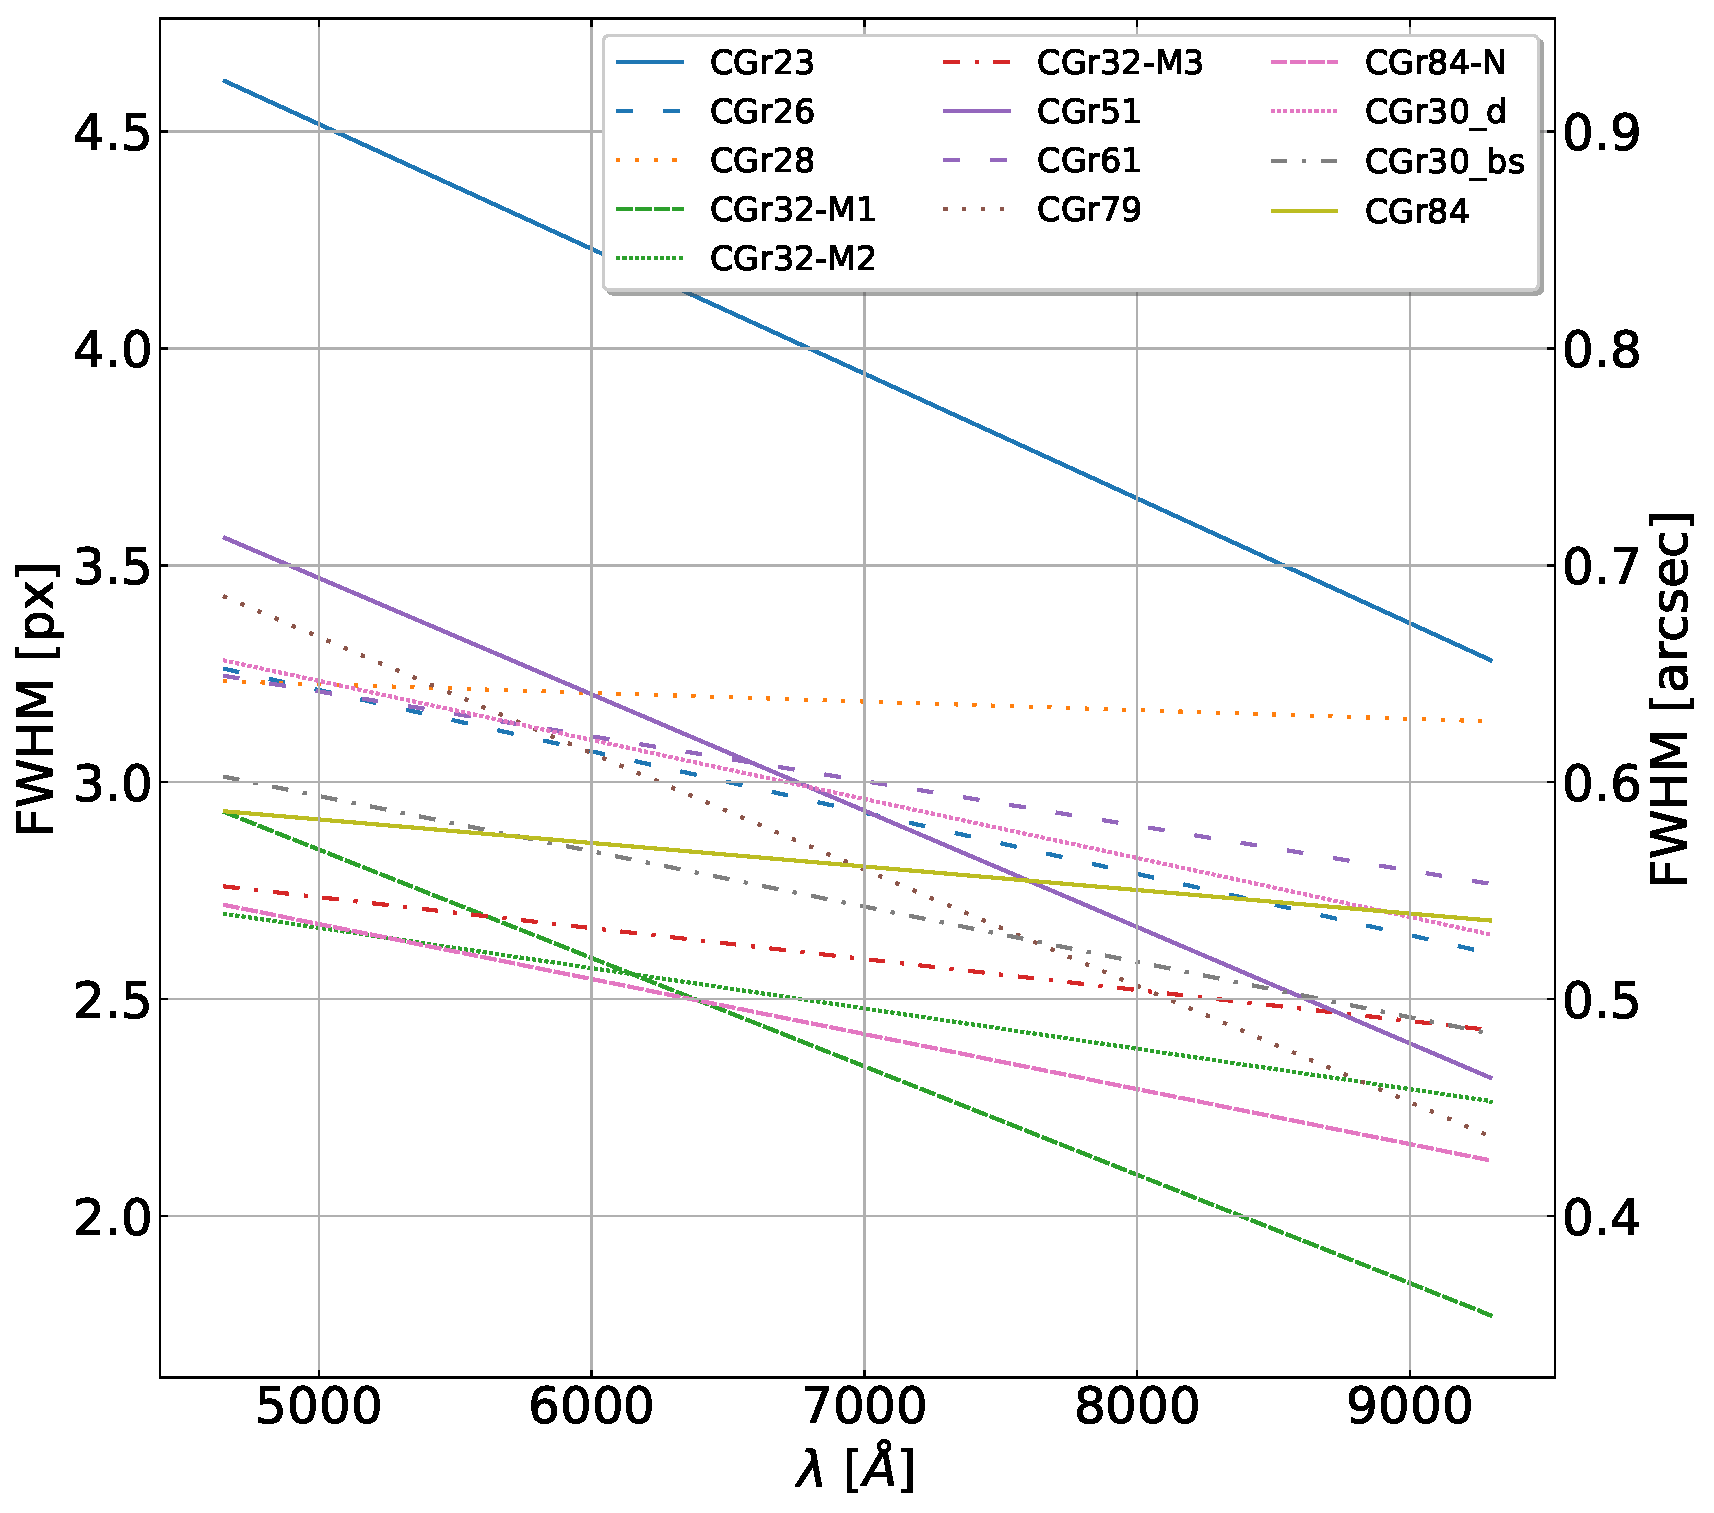
\includegraphics[width=\linewidth]{../Plots/FWHM_variation_with_lambda.pdf}
	\caption[PSF FWHM variation with wavelength.]{PSF FWHM variation with wavelength for the 13 FoVs as measured by Valentina. At least two values of the FWHM were derived from stars in the FoVs by fitting a Moffat distribution to their light profile. We assumed a linear evolution with wavelength. Strong fluctuations appear depending on the observed FoV.}
	\label{fig:FWHM_var_lambda}
\end{figure}

Since we are interested in keeping well resolved field galaxies, we need to apply relevant criteria in order to select the right galaxies. The most obvious parameter we can use to make our selection is the size of the galaxy, though we must be certain before using it that the value given in our cross-matched catalogue reflects accurately enough the "true" size of the galaxy. This checking is performed and discussed in the next section.

Following the earlier work done in \shortciteA{Bacon2015} and \shortciteA{Bacon2017}, the MUSE Point Spread Function (PSF), that is the pattern we obtain when we observe a point-like source with MUSE, is most well described by a \shortciteA{MoffatProfile} profile

\begin{equation}
	I_{\rm{PSF}}(r) = I_0 (1 + (r/\alpha)^2 ) ^{- \beta}
\end{equation}
where $r$ is the radial distance to the centre and $\alpha$, $\beta$ are two seeing dependant parameters. In our case we are interested in the Full Width at Half Maximum (FWHM) since it is directly related to the seeing conditions and it gives us information about the minimum spatial extent within which data will be mixed up.
The FWHM can be easily derived from the equation $I_{\rm{PSF}} ( \rm{FWHM}/2) = I_0 /2$, from which we get the following relation

\begin{equation}
	\rm{FWHM} = 2 \alpha \sqrt{2^{1/\beta} - 1 }
\end{equation}

According to the aforementioned articles the value of $\beta$ should remain roughly constant and we would expect from differential image motion theory (insert this paper here when read 10.1086/342683) that the FWHM  would linearly decrease with wavelength. Thus, if we want to derive the FWHM at a given wavelength and in a given field (since the seeing conditions will vary with the date of observation) we need to derive the linear relation between the FWHM and the wavelength in each field.

The measure of $\alpha$, and therefore the FWHM, was done by Valentina on at least two stars by FoV. Because they belong to our galaxy, we can consider that they have a null redshift, so that the wavelength of observation and emission are the same.

 A Moffat profile was fitted on their OII $\lambda \SI{3727}{\angstrom}$ and OIII $\SI{5007}{\angstrom}$ flux maps, giving us at least two measures of the FWHM . Though a more rigorous modelling of the wavelength variation of the PSF FWHM including both more data points and potentially higher order terms is mandatory for future analysis, we decided to stick to this values in the present work, keeping in mind the large uncertainties which will affect the velocity dispersion maps in the modelling section. A representation of the FWHM variation with wavelength for 13 out of 16 observations is shown in Fig.\,\ref{fig:FWHM_var_lambda}. We have missing values of the FWHM for groups CGr34 (2 observations, 1 deep and 1 best-seeing) and CGr114. There appear to have a strong variations given the time of observation, up to $\SI{0.7}{arcsec}$. \\
 
Having computed the PSF FWHM  linear relation with wavelength for each FoV, we are now able to derive the relevant value of the FWHM for galaxies at any redshift. Indeed, since all our observations are limited to the OII $\lambda \SI{3727}{\angstrom}, \SI{3729}{\angstrom}$ doublet, we can derive the wavelength of observation for each galaxy given its redshift with the usual relation

\begin{equation}
	\lambda_{\rm{obs}} = \lambda_{\rm{em}} ( 1 + z )
\end{equation}
where $z$ is the redshift or the galaxy and $\lambda_{\rm{em}}$, $\lambda_{\rm{obs}}$ respectively the emitted (rest-frame) and observed wavelengths, and we can use this value to find the FWHM.\\

Considering that the FWHM is a measure of how spread a point-like source is in our images, and since we are interested in working with resolved enough galaxies in order to better constrain their kinematics, we would like galaxies to have a characteristic size at least above the FWHM. The only size which is given in the morphological catalogues is the half-light radius derived from optical images. 

According to \shortciteA{Swinbank2017} who compared the half-light radius of the nebular OII emission in MUSE images with that of their HST counterpart in ACS \textit{I} or WFC \textit{H}-band, the OII half-light radius seems to scale with the HST radius as 

\begin{equation}
	R_{1/2}^{\rm{OII}} = (1.18 \pm 0.03) R_{1/2}^{\rm{HST}}
\end{equation}

Thus, choosing the FWHM as a lower limit for the morphological radius in our sample should get rid ourselves of most of unresolved galaxies without removing too many "good" galaxies. This is checked in the next sections.

\subsubsection{SNR selection}

The other information we can use to select our sample is the Signal to Noise Ratio (SNR), which tells us how well our galaxy is detached from the background. The SNR is generally derived as the ratio between the source's signal and the background level. The noisier an image, the lower the SNR is, which explains the need of a good data reduction pipeline.

As described in later sections, the galaxies must be automatically and then manually cleaned before fitting a kinematical model on the velocity maps in order to remove any noise dominated pixel which might compromise the fit. One of the criteria used by the routine to decide whether a pixel belongs to the galaxy or is noise-dominated is a lower limit on SNR (typically $5$). Thus, if we want to have enough detection in our cleaned maps to perform the kinematical modelling, we must select galaxies with a strong enough SNR.

In our case, \textsc{CAMEL}\footnote{\url{https://bitbucket.org/bepinat/camel/src/master/}} software, described in \shortciteA{Epinat2012}, was used on the integrated spectrum in order to derive spectral features of the galaxies. We used the OII flux and its error to derive the SNR as

\begin{equation}
	\rm{SNR} = \frac{\rm{OII \,\, flux}}{\rm{OII \,\, flux \,\, error}}
\end{equation}

This represents the OII SNR computed from the integrated galaxy spectrum using pixels within the smaller data cube centred around the galaxy. Since the typical SNR value used by the routine to clean the maps is around $5$, we decided as a first step to choose an SNR lower limit of $10$, allowing us to keep galaxies with strong enough detection after the automatic cleaning.

\subsubsection{Selection criteria}

To summarize, we decided to apply the two following cuts (lower limits):

\begin{itemize}
	\item $R_{1/2 , \rm{lim}} = \rm{FWHM} \approx \SI{0.7}{arcsec}$
	\item $\rm{SNR_{lim}} = 10$
\end{itemize}

It should be emphasized that these selection criteria should be used in combination rather than alone. Indeed, having a potentially large galaxy does not prevent us from having a low SNR per pixel, resulting in a too small cleaned galaxy for the kinematical modelling. In the same way, a high SNR could be obtained for a small galaxy, and we expect them to appear much larger in MUSE images because of beam smearing effects.





 
